In this section an STFT will be implemented in Python and tested to check that it fulfils the test criteria specified in chapter \ref{ch3}. This includes creating a spectrogram from the results of the STFT and check if this is consistent with the expected results. The implementation is based on the theory of the discrete STFT described in section \ref{sec:STFT}.

\subsection{Implementation of the STFT and spectrogram}
The implementation of the STFT requires an FFT algorithm and will use the algorithm described in algorithm \ref{FFTalg}. The algorithm for the implementation is seen below in algorithm \ref{STFTalg}. The Hann window is used as an example window but is later compared to other windows, and an overlap of 50\% is decided due to the conventional usage of this. The overlap specifies the overlap of two adjacent windows.
\begin{algorithm}[H]
\caption{STFT algorithm}
\label{STFTalg}
\begin{algorithmic}[1]
\State $FFTsize=2^{l}$ \Comment{Length of window and FFT in STFT}
\State $overlap=2$ \Comment{Overlaps of every FFT - 2 is 50\% overlap of adjacent windows}
\State $data = filename.wav$ \Comment{Recording imported as .wav file}\\
\Procedure{Compute STFT}{$FFTsize,overlap,data$}
\State $step=FFTsize/overlap$
\State $w=hanning(FFTsize)$ \Comment{Hanning window of length $=FFTsize$}
\For{each $i$ at intervals of $step$ in length of $data-FFTsize$}
\State $stft = array[FFT(w\cdot data[i:i+FFTsize])]$
\EndFor
\State Return $stft$
\EndProcedure
\end{algorithmic}
\end{algorithm}
The algorithm for generating a spectrogram from the STFT is seen in algorithm \ref{SPECTROalg}.
\begin{algorithm}[H]
\caption{Generate spectrogram}
\label{SPECTROalg}
\begin{algorithmic}[1]
	\State $X=STFT(FFTsize,overlap,data)$ 					\Comment{Perform STFT on data}
	\Procedure{Spectrogram}{$X,f_s$}
	\State $time=len(data)/f_s$ \Comment{Length of 		data in seconds.}
	\State $X=20\cdot \log_{10}(abs(X.T))$ \Comment{dB 	gain of transposed $stft$}\\
	\State $x=linspace(0,time,len(X[1]))$ 		\Comment{Ticks 		for x-axis}
	\State $y=linspace(0,f_s/2,len(X[0]))$ 	\Comment{Ticks 	for y-axis}\\
	\Return $x$, $y$
\EndProcedure
\end{algorithmic}
\end{algorithm}

\subsection{Validation of the STFT and spectogram}
The validation of the STFT and spectrograms will be done as a whole entity, and the test specification consists of generating a spectrogram from a discrete signal. The discrete signal to be used is\frede{Lav det her om til et kontinuert signal}
\begin{align}\label{eq:SPECTROsignal}
sig[n]=\begin{cases}\sin(1000\pi n)&\text{for }0\leq n<\frac{75}{3}\\
\sin(3000\pi n)&\text{for }\frac{75}{3}\leq n < \frac{150}{3}\\
\sin(3000\pi n)+\sin(3250\pi n)&\text{for }\frac{2t}{3}\leq n\leq\frac{2t}{3}
\end{cases}
\end{align}
The sine waves are then with frequencies of 500, 1500 and 1625 Hz, respectively, and the signal is sampled at $f_s=4000$ Hz. Figure \ref{fig:test_stft} shows spectrograms of the signal generated with windows of different lengths.
\begin{figure}[H]
\centering
\begin{subfigure}{0.49\textwidth}
\centering
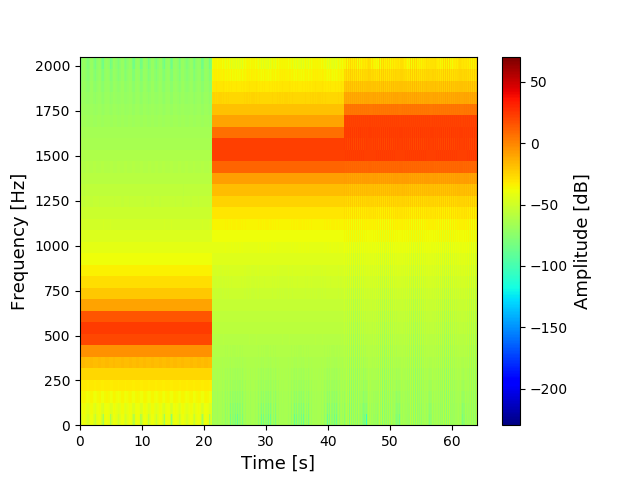
\includegraphics[width=\textwidth]{figures/validation/stft/1.png}
\caption{}
\label{fig:test_stft2}
\end{subfigure}
\begin{subfigure}{0.49\textwidth}
\centering
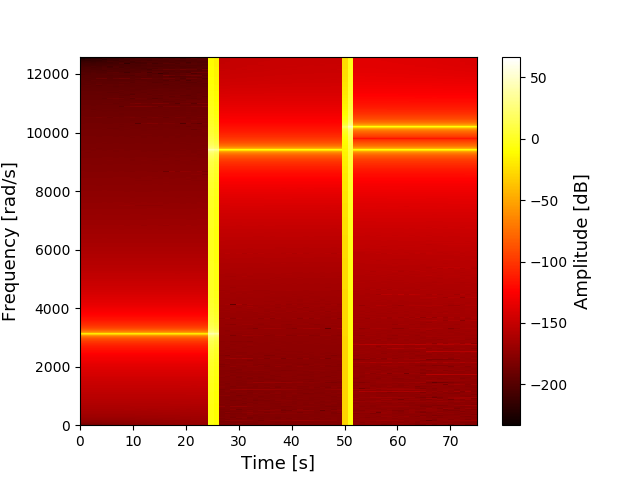
\includegraphics[width=\textwidth]{figures/validation/stft/2.png}
\caption{}
\label{fig:test_stft1}
\end{subfigure}
\caption{\textbf{(a)}Spectrogram of signal in \eqref{eq:SPECTROsignal} generated with a Hann window of length $2^6=64$ and overlap of 2. The low spectral and high temporal resolutions follow from a narrow window used in the STFT. \textbf{(b)} Spectrogram of signal in \eqref{eq:SPECTROsignal} generated with a Hann window of length $2^{13}=8192$ and overlap of 2. The high spectral and low temporal resolutions follow from a wide window used in the STFT.}
\label{fig:test_stft}
\end{figure}
From figure \ref{fig:test_stft} it is clearly seen how the length of the window in the STFT used for generating the spectrogram affects the resolution in time and frequency. This agrees with Heisenberg's uncertainty principle described in section \ref{sec:heisenberg}. By figure \ref{fig:test_stft} it is concluded that the implementations of the STFT and spectrogram work as intended. Further optimisation is possible through the type and length of window used in the STFT.

\subsection{Variation of windows in STFT}\label{sec:STFT_variation}
The STFT uses a window function to taper the segment of the data to be transformed, and different windows produce different results. Figure \ref{fig:stft_windows_10000} shows spectrograms of the test signal generated from different windows of length $2^{13}=8192$. Similarly, figure \ref{fig:stft_windows_100} shows spectrograms from STFTs with windows of length $2^6=64$.
\begin{figure}[H]
\centering
\begin{subfigure}{0.49\textwidth}
\centering

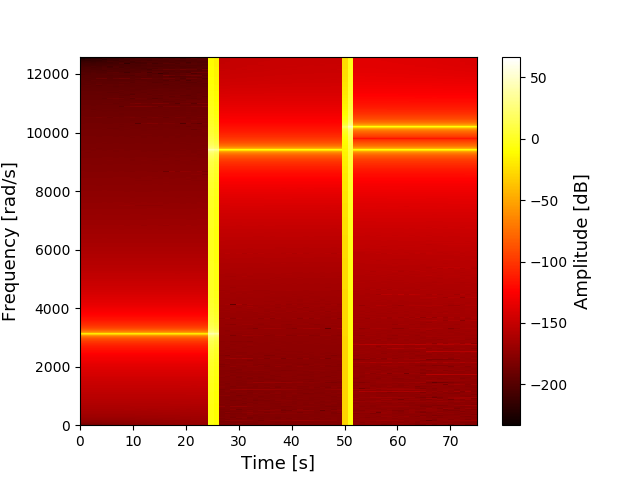
\includegraphics[width=\textwidth]{figures/stft_windows/hanning_10000.png}
\caption{Hann window.}
\label{fig:stft_hanning}
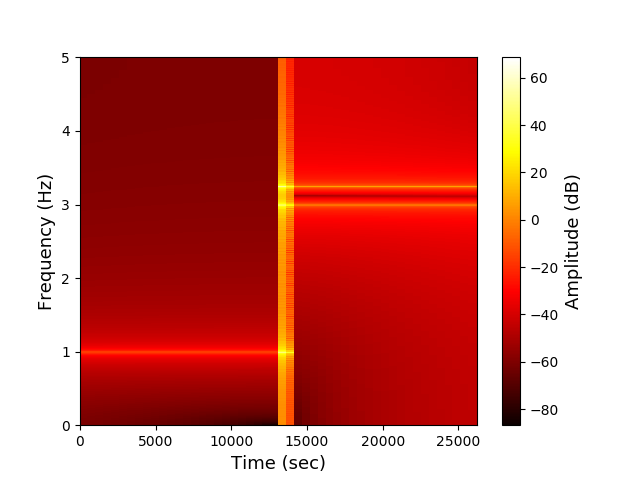
\includegraphics[width=\textwidth]{figures/stft_windows/hamming_10000.png}
\caption{Hamming window.}
\label{fig:stft_hamming}
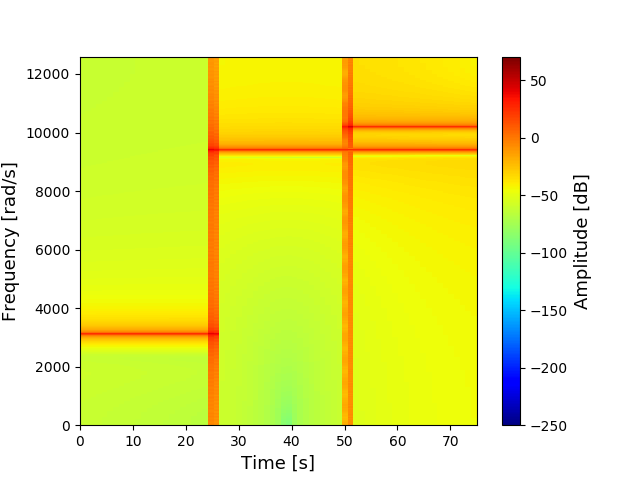
\includegraphics[width=\textwidth]{figures/stft_windows/kaiser/10000/4.png}
\caption{Kaiser window, $\beta=4$.}
\label{fig:stft_kaiser_10000_4}
\end{subfigure}
\centering
\begin{subfigure}{0.49\textwidth}
\centering

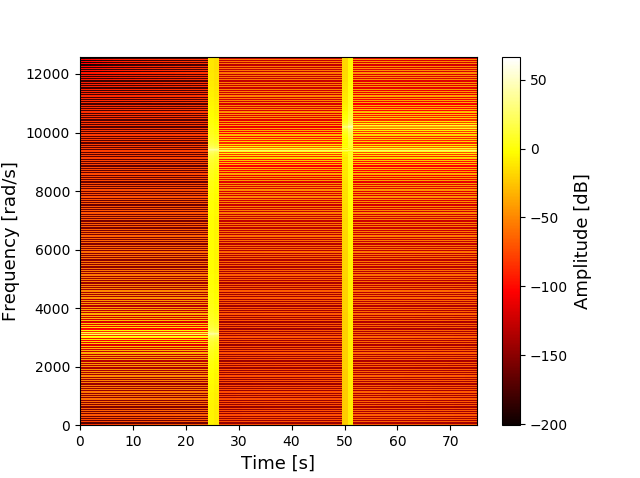
\includegraphics[width=\textwidth]{figures/stft_windows/bartlett_10000.png}
\caption{Bartlett window.}
\label{fig:stft_bartlett}
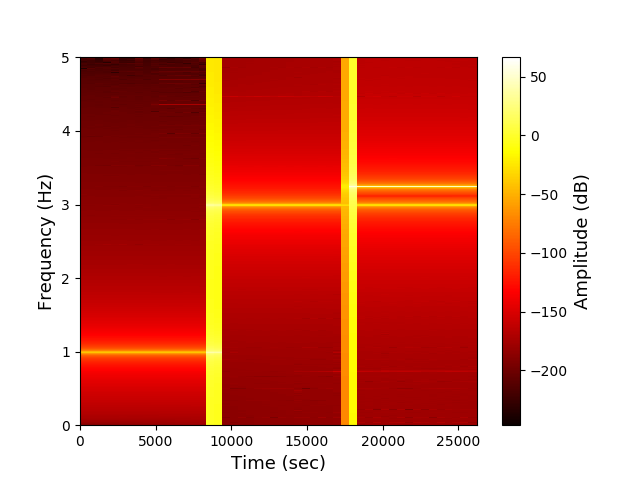
\includegraphics[width=\textwidth]{figures/stft_windows/blackman_10000.png}
\caption{Blackman window.}
\label{fig:stft_blackman}
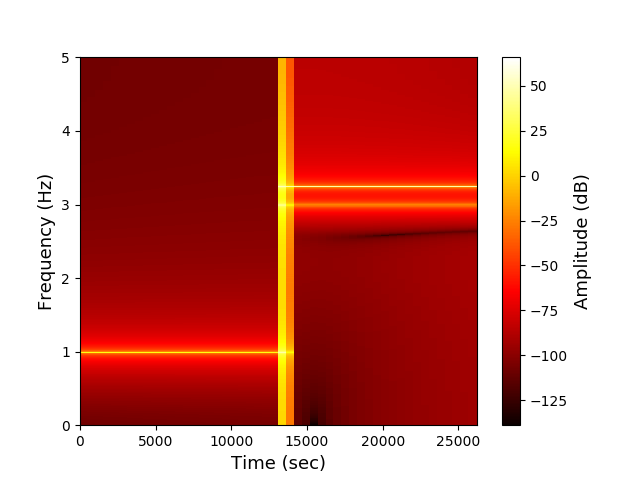
\includegraphics[width=\textwidth]{figures/stft_windows/kaiser/10000/10.png}
\caption{Kaiser window, $\beta=10$.}
\label{fig:stft_kaiser_10000_10}
\end{subfigure}

\caption{Spectrograms generated with different windows of length $2^{13}$ and with overlap of 50\%.}
\label{fig:stft_windows_10000}
\end{figure}

\begin{figure}[H]
\centering
\begin{subfigure}{0.49\textwidth}
\centering
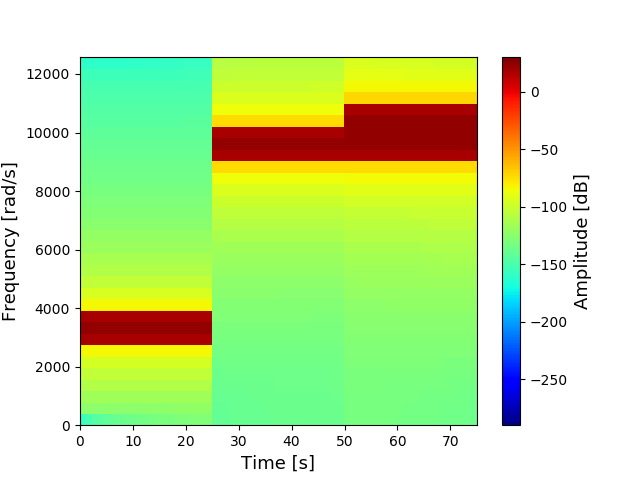
\includegraphics[width=\textwidth]{figures/stft_windows/100/hanning.png}
\caption{Hann window.}
\label{fig:stft_hanning_100}
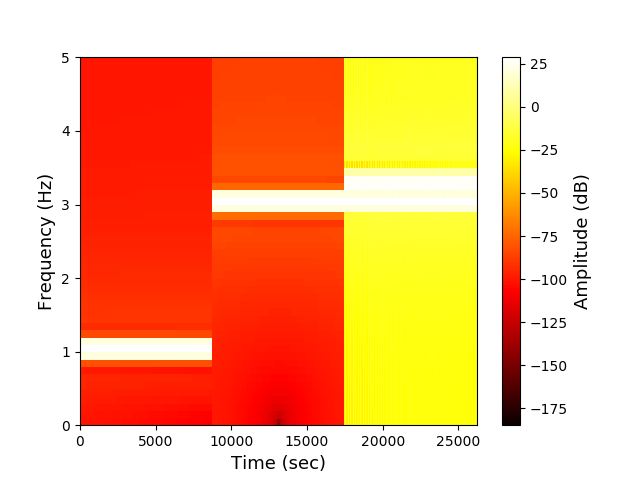
\includegraphics[width=\textwidth]{figures/stft_windows/100/hamming.png}
\caption{Hamming window.}
\label{fig:stft_hamming_100}
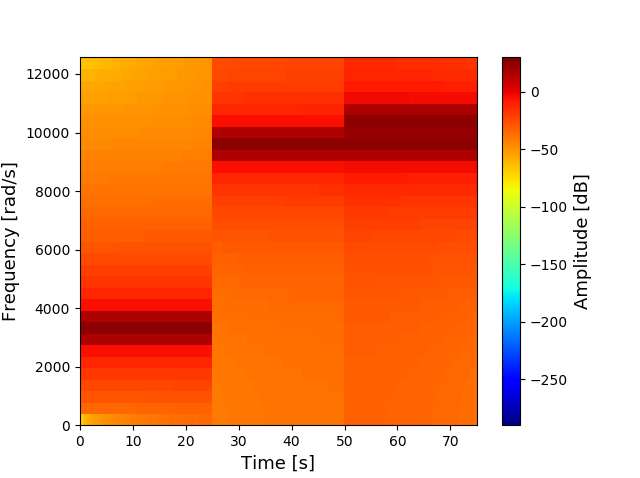
\includegraphics[width=\textwidth]{figures/stft_windows/100/kaiser_4.png}
\caption{Kaiser window, $\beta=4$.}
\label{fig:stft_kaiser_100_4}
\end{subfigure}
\begin{subfigure}{0.49\textwidth}
\centering
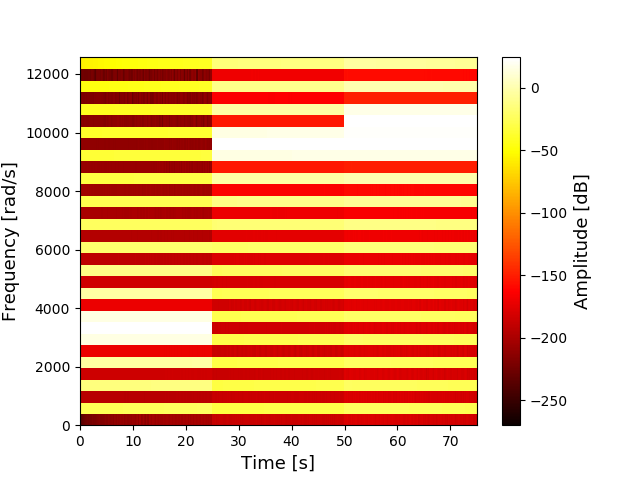
\includegraphics[width=\textwidth]{figures/stft_windows/100/bartlett.png}
\caption{Bartlett window.}
\label{fig:stft_bartlett_100}
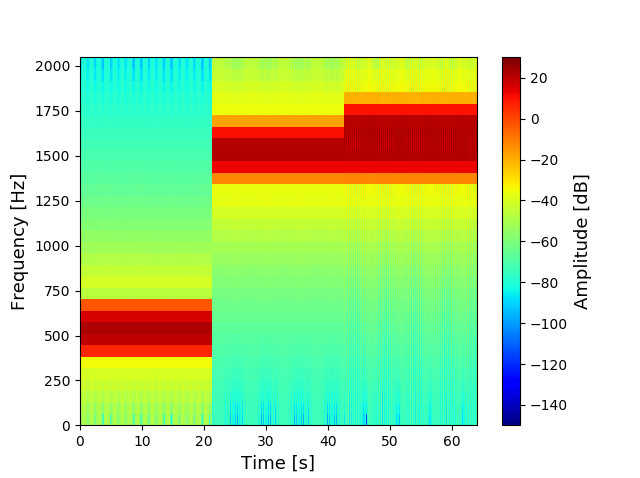
\includegraphics[width=\textwidth]{figures/stft_windows/100/blackman.png}
\caption{Blackman window.}
\label{fig:stft_blackman_100}
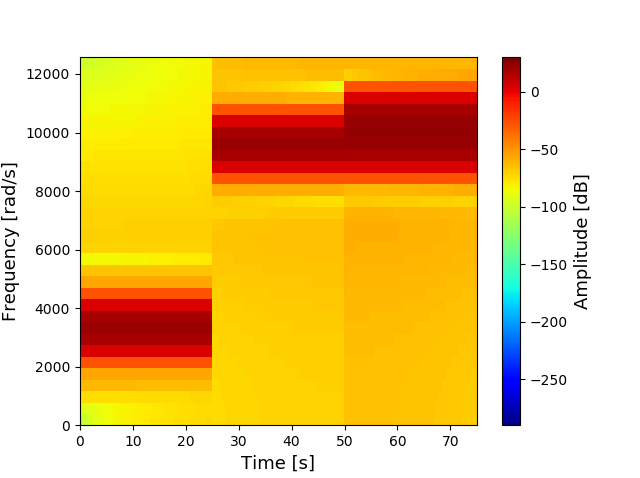
\includegraphics[width=\textwidth]{figures/stft_windows/100/kaiser_10.png}
\caption{Kaiser window, $\beta=10$.}
\label{fig:stft_kaiser_100_10}
\end{subfigure}
\caption{Spectrograms generated with different windows of length $2^6$ and with overlap of 50\%.}
\label{fig:stft_windows_100}
\end{figure}
\subsection{Peak detection under varying window orders}
As the goal of the project is to be able to detect the most significant frequencies in a piece of music from the generated spectrogram it is in this section tested how the order $M$ of the window used in the STFT affects a peak detection algorithm's ability to do so. The algorithm used to detect the most significant frequencies is explained and implemented in section \ref{sec:peak_detection}. The goal is to decide when the peak algorithm no longer detects the most significant frequencies in the signal as a result of bad spectral resolution. From this the minimum required order $M$ of the window in the STFT can be specified.\\\\
In figure \ref{fig:2048spec} is seen the spectrogram of \ref{eq:SPECTROsignal} generated with a Hann window of order $M=2^{11}$ as well as the associated results of the peak detection algorithm in figure \ref{fig:2048peak}. Likewise figure \ref{fig:1024spec}  shows the spectrogram of \eqref{eq:SPECTROsignal} generated with a Hann window of order $M=2^{10}$ with the associated peak detection in figure \ref{fig:1024peak}.
\begin{figure}[H]
\centering
\begin{subfigure}{0.49\textwidth}
\centering
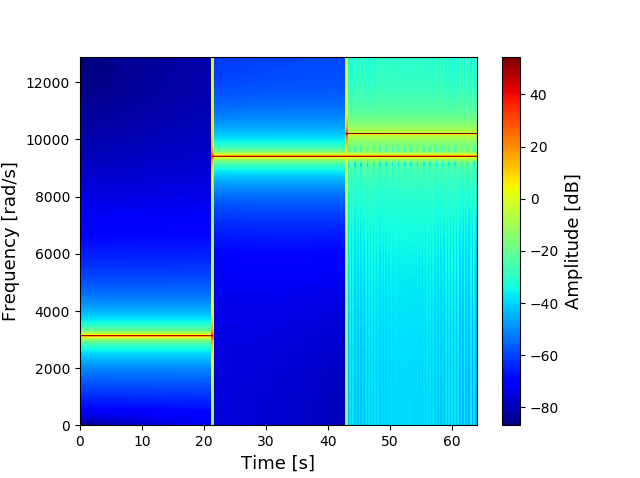
\includegraphics[width=\textwidth]{figures/validation/stft/peak/spectro2048.png}
\caption{}
\label{fig:2048spec}
\end{subfigure}
\begin{subfigure}{0.49\textwidth}
\centering
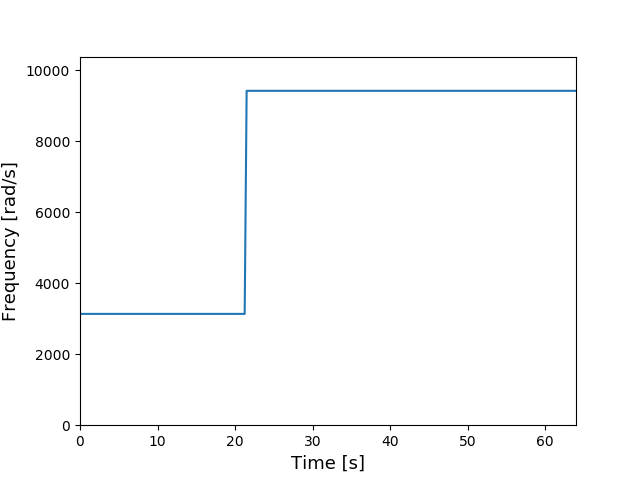
\includegraphics[width=\textwidth]{figures/validation/stft/peak/peak2048.png}
\caption{}
\label{fig:2048peak}
\end{subfigure}
\caption{\textbf{(a)} Spectrogram of \eqref{eq:SPECTROsignal} generated with a Hann window of order $M=2^{11}$. \textbf{(b)} Peak detection of spectrogram.}
\label{fig:2048}
\end{figure}
\begin{figure}[H]
\centering
\begin{subfigure}{0.49\textwidth}
\centering
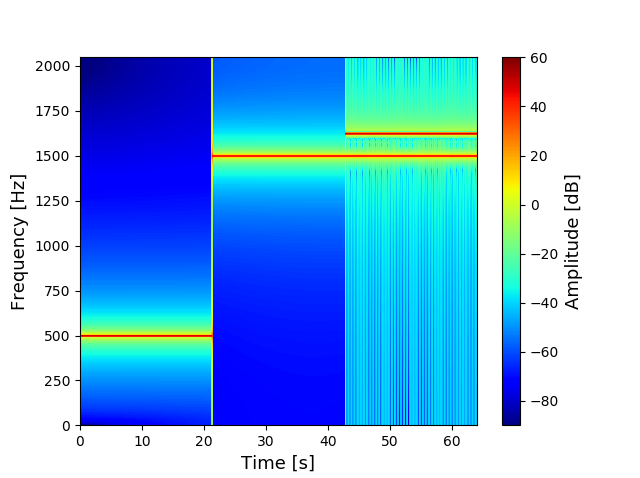
\includegraphics[width=\textwidth]{figures/validation/stft/peak/spectro1024.png}
\caption{}
\label{fig:1024spec}
\end{subfigure}
\begin{subfigure}{0.49\textwidth}
\centering
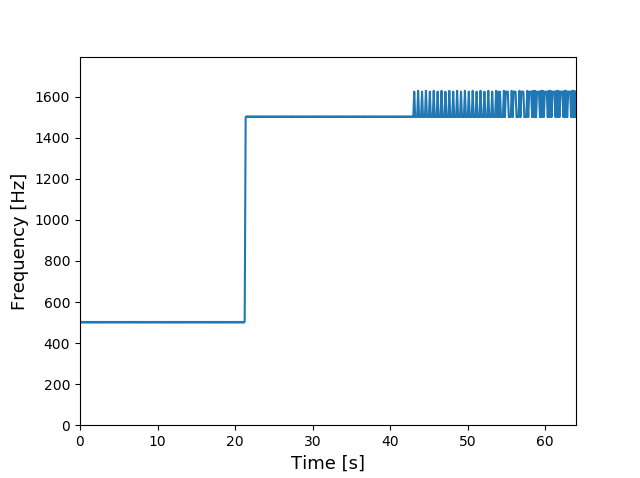
\includegraphics[width=\textwidth]{figures/validation/stft/peak/peak1024.png}
\caption{}
\label{fig:1024peak}
\end{subfigure}
\caption{\textbf{(a)} Spectrogram of \eqref{eq:SPECTROsignal} generated with a Hann window of order $M=2^{10}$. \textbf{(b)} Peak detection of spectrogram.}
\label{fig:1024}
\end{figure}
From figure \ref{fig:1024} it is seen that a Hann window of order $M=2^{10}$ does not produce a spectral resulution sufficient for the peak detection algorithm to detect the most significant frequency but jumps between different frequencies. Figure \ref{fig:2048} shows $M=2^{11}$ is sufficient for the peak detection algorithm. It can be concluded that the order $M$ of the window used in the STFT should be at least $2^{11}$.
\subsection{Summary}
Fredric J. Harris wrote an article in 1978 analysing the different windows and their effects in signal processing with the discrete Fourier transform \cite{page 82, fredric_harris}. His analysis included quantative and qualitative arguments, and he ends the article concluding that the Kaiser and Blackman windows are the best choices for this kind of signal processing his favourite being the Kaiser window. It is furthermore assessed from the above spectrograms, which allow for a visual (and qualitative) analysis, that the Kaiser window produces the best looking spectrograms. Together with the conclusion from Harris it is decided that a Kaiser window of order $M=2^{12}$ with shape coefficient $\beta = 6$ will be used for the implementation of the STFT in this project as it produces a sufficient spectral resolution for peak detection and good looking spectrograms.\\
Figure \ref{fig:STFT_test_signal} shows the resulting STFT of an octatonic scale played on a guitar one string at a time with the use of a Kaiser window of order $2^{12}$ and $\beta = 6$.

\begin{figure}[H]
\centering
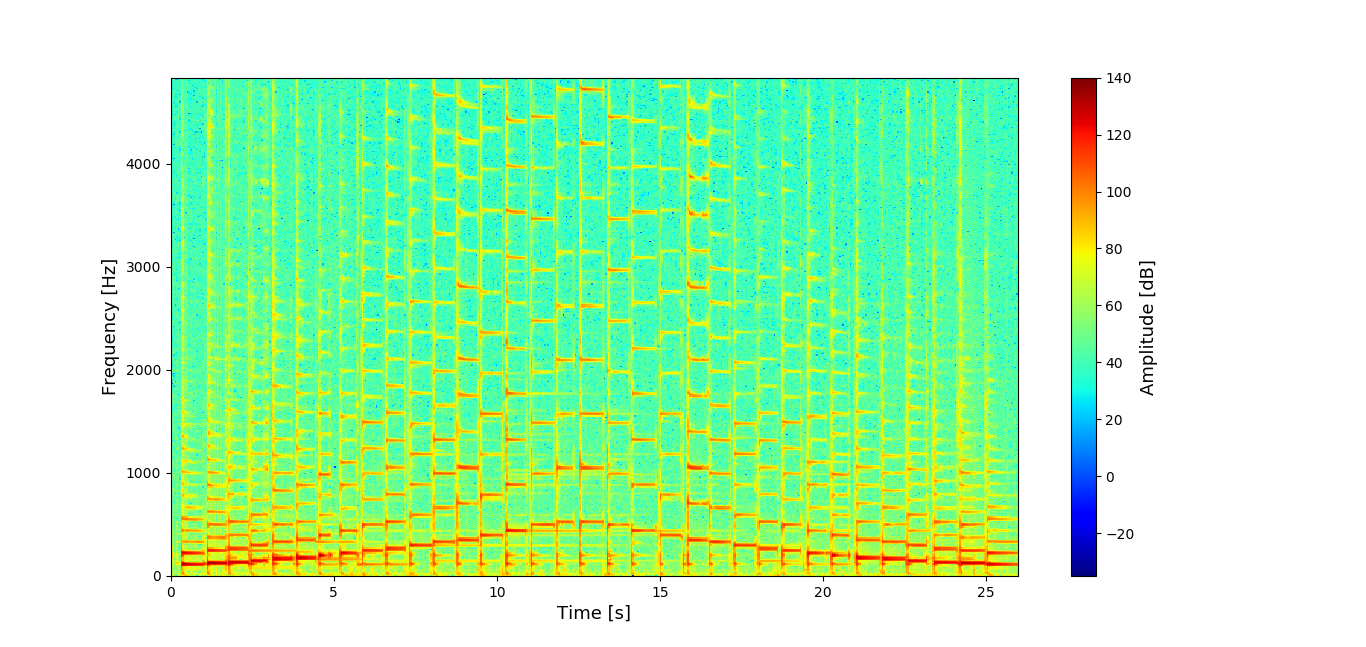
\includegraphics[width = 1.1\textwidth]{figures/validation/stft/scale.png}
\caption{Spectrogram of octatonic scale plucking only one string at a time. STFT computed by use of Kaiser window of order $2^{12}$ and $\beta = 6$.}
\label{fig:STFT_test_signal}
\end{figure}